\apendice{Plan de Proyecto Software}

\section{Introducción}

El plan de proyecto presenta al lector un estudio del proceso organizativo y de gestión seguido a lo largo del desarrollo del proyecto con el propósito de cumplir con los objetivos propuestos dentro de los plazos establecidos. 

En los siguientes apartados se detallan los aspectos relativos a la distribución de las tareas, el estudio de los gastos asumidos durante la realización del proyecto y los aspectos legales relativos a la propiedad intelectual de los ficheros del proyecto, incluyendo su documentación y dependencias.


\section{Planificación temporal}

La planificación de temporal de los objetivos del proyecto se ha realizado siguiendo las recomendaciones de la metodología ágil SCRUM. La base de esta metodología consta de la realización periódica de reuniones que permitan mantener un control sobre el progreso en las tareas propuestas para cada Sprint.

Estas reuniones coincidirían con la finalización de cada Sprint y constarían de dos partes. Una primera parte se centraría en la finalización del Sprint, donde se trataría de presentar los avances realizados en los objetivos, se presentarían los problemas encontrados y las soluciones propuestas para su resolución. En la segunda parte se propondrían las tareas y planificación del siguiente Sprint a partir de la retroalimentación obtenida por los tutores del proyecto.

\subsection{Sprint 1: Toma de Contacto}

El sprint inicial tuvo lugar tras la aprobación del proyecto. Durante la reunión inicial se establecieron algunos de los objetivos generales que se perseguían con su realización. Partiendo de cero se propuso llevar a cabo el desarrollo mediante el uso de Python debido a que se disponía de un mayor conocimiento en dicho lenguaje. 

Uno de los objetivos principales del proyecto sería trabajar con datos extraídos de la plataforma GitHub. Durante este sprint se decidió realizar un prototipo que permitiese llevar a cabo la descarga de información de repositorios públicos mediante el uso de la API REST de GitHub. Para ello se localizaron módulos de Python que simplificaban el proceso de realización de llamadas a GitHub y el tratamiento de la información recibida. Se realizó un estudio del funcionamiento de las diversas alternativas hasta seleccionar el paquete más se adaptase a las necesidades del proyecto de acuerdo con la calidad de su implementación y la disponibilidad de una documentación adecuada.

\subsubsection{Listado de tareas}

\begin{itemize} \setlength\itemsep{0.2em}
    \item \href{https://github.com/MrpYA45/github-text-mining-tfg/issues/1}{Investigar sobre la conexión con GitHub} [3h].
    \item \href{https://github.com/MrpYA45/github-text-mining-tfg/issues/3}{Prototipar la descarga de issues mediante PyGithub} [3h].
    \item \href{https://github.com/MrpYA45/github-text-mining-tfg/issues/4}{Testear las limitaciones de la API de GitHub} [2h].
\end{itemize}

\subsection{Sprint 2: Primera iteración de la extracción y almacenamiento de la información.}

El segundo sprint del proyecto contempla la planificación de la arquitectura del proyecto con la finalidad de diseñar una arquitectura de microservicios de acuerdo con los objetivos del proyecto. Para ello, se realizó un estudio de los servicios requeridos para cumplir con las funcionalidades previstas de la aplicación y la forma de mantener la comunicación entre ellos.

Una vez se tomaron estas decisiones se dio comienzo al diseño e implementación de la estructura de la base de datos a través del mapeo de objetos relacionales mediante el uso del paquete SQLAlchemy. Este paquete actuaría como dependencia del servicio principal en cada uno de los servicios, permitiendo su acceso al contenido de la base de datos.

\subsubsection{Listado de tareas}

\begin{itemize} \setlength\itemsep{0.2em}
    \item \href{https://github.com/MrpYA45/github-text-mining-tfg/issues/6}{Realizar el cambio de biblioteca que maneja la conexión con GitHub} [2h].
    \item \href{https://github.com/MrpYA45/github-text-mining-tfg/issues/8}{Crear un prototipo para la base de datos} [10h].
    \item \href{https://github.com/MrpYA45/github-text-mining-tfg/issues/7}{Crear un administrador para la descarga de los repositorios} [10h].
    \item \href{https://github.com/MrpYA45/github-text-mining-tfg/issues/9}{Tratamiento de las excepciones de la base de datos y de la extracción de GitHub} [3h].
\end{itemize}

\subsection{Sprint 3: Primera iteración de la API REST y concurrencia.}

En este tercer sprint se realizó la primera implementación del servicio de API REST junto a un pequeño front-end que permitiría realizar una serie de comprobaciones básicas. También se desarrollarían una serie de scripts que permitirían automatizar la detección y comprobación de errores de tipado por medio de las GitHub Actions. De manera paralela se realizó un estudio de las posibilidades de implementar la concurrencia en la descarga de los repositorios.

\subsubsection{Listado de tareas}

\begin{itemize} \setlength\itemsep{0.2em}
    \item \href{https://github.com/MrpYA45/github-text-mining-tfg/issues/11}{Estudiar la aplicación de concurrencia en Python} [6h].
    \item \href{https://github.com/MrpYA45/github-text-mining-tfg/issues/13}{Implementar las Acciones de GitHub para la comprobación de tipado y estilo} [2h].
    \item \href{https://github.com/MrpYA45/github-text-mining-tfg/issues/14}{Primera implementación básica de Flask } [4h].

\end{itemize}

\subsection{Sprint 4: Microservicios y Flask}

En este cuarto sprint se diseño una configuración de Docker que permitiría el despliegue de la aplicación en un contenedor propio. Para adaptar la aplicación a Docker se realizó una reorganización de los paquetes y se diseñaron una serie de scripts que permitirían lanzar los servicios automáticamente al arrancar los contenedores.

\subsubsection{Listado de tareas}

\begin{itemize} \setlength\itemsep{0.2em}
    \item \href{https://github.com/MrpYA45/github-text-mining-tfg/issues/10}{Documentación del código de la capa de datos y la capa lógica} [4h].
    \item \href{https://github.com/MrpYA45/github-text-mining-tfg/issues/2}{Explorar la organización de la arquitectura de microservicios } [6h].
    \item \href{https://github.com/MrpYA45/github-text-mining-tfg/issues/17}{Creación de scripts bash que permitan la instalación y ejecución de la aplicación} [4h].
    \item \href{https://github.com/MrpYA45/github-text-mining-tfg/issues/16}{Rediseño del software - Diseño evolutivo} [5h].
    \item \href{https://github.com/MrpYA45/github-text-mining-tfg/issues/15}{Implementación de Docker para el despliegue de la aplicación. } [3h].

\end{itemize}

\subsection{Sprint 5: Primera iteración del servicio de procesamiento.}

Este quinto sprint se logró implementar la primera aproximación del servicio de procesamiento incluyendo el modelo de clasificación Zero-Shot. También se actualizó el servicio de extracción para contemplar la recogida de las etiquetas del repositorio.

\subsubsection{Listado de tareas}

\begin{itemize} \setlength\itemsep{0.2em}
    \item \href{https://github.com/MrpYA45/github-text-mining-tfg/issues/21}{Mejora y adición de métodos para poder introducir el procesamiento } [6h].
    \item \href{https://github.com/MrpYA45/github-text-mining-tfg/issues/22}{Recoger los datos de las etiquetas de los repositorios} [4h].
    \item \href{https://github.com/MrpYA45/github-text-mining-tfg/issues/23}{Implementar modelo NLP Zero Shot Classifier } [8h].

\end{itemize}
 
\subsection{Sprint 6: Segunda iteración del servicio de procesamiento.}

En este sexto sprint adoptó el lanzamiento de los diferentes servicios que componen la aplicación en contenedores separados a través de docker-compose, de esta manera los servicios podrían mantenerse aislados los unos de los otros.

\subsubsection{Listado de tareas}

\begin{itemize} \setlength\itemsep{0.2em}
    \item \href{https://github.com/MrpYA45/github-text-mining-tfg/issues/25}{Separación de módulos en diferentes contenedores mediante docker-compose} [12h].
    \item \href{https://github.com/MrpYA45/github-text-mining-tfg/issues/28}{Añadir la detección y descarga automática de modelos cuando no se posean} [4h].
\end{itemize}

\subsection{Sprint 7: Actualización de la base de datos e introducción de los ficheros de configuración.}

En este séptimo sprint se decidió reemplazar el uso SQLite como gestor de base de datos por MariaDB debido a los problemas de concurrencia derivados del aislamiento de los servicios en distintos contenedores. En el servicio de procesamiento se implementó un sistema encargado de descargar los modelos desde Hugging Face de manera que mantuviesen de forma local en el equipo.

\subsubsection{Listado de tareas}

\begin{itemize} \setlength\itemsep{0.2em}
    \item \href{https://github.com/MrpYA45/github-text-mining-tfg/issues/27}{Crear/Actualizar el fichero de configuración por módulo} [4h].
    \item \href{https://github.com/MrpYA45/github-text-mining-tfg/issues/26}{Cambiar la base de datos de SQLite a MariaDB } [8h].
\end{itemize}

\subsection{Sprint 8: Tercera iteración del servicio de procesamiento.}

En este octavo sprint se centra en la implementación de estrategias que permitan someter a la información extraída a un preprocesado donde se eliminen las impurezas de los datos con el objetivo de mejorar los resultados de los modelos.

En adición a estas estrategias, se tomó como referencia los algoritmos de división de textos y optimización del contexto implementados en el proyecto <<JIZT>> buscando obtener mejores resultados ante entradas de los modelos que superasen las limitaciones relativas al tamaño de las entradas de los modelos.

\subsubsection{Listado de tareas}

\begin{itemize} \setlength\itemsep{0.2em}
    \item \href{https://github.com/MrpYA45/github-text-mining-tfg/issues/29}{Creación de utilidades para el tratamiento de la información extraída} [6h].
    \item \href{https://github.com/MrpYA45/github-text-mining-tfg/issues/30}{Implementación de algoritmos de sección y balanceo de textos} [15h].
    \item \href{https://github.com/MrpYA45/github-text-mining-tfg/issues/34}{Almacenamiento de los resultados de los modelos} [15h].
    \item \href{https://github.com/MrpYA45/github-text-mining-tfg/issues/31}{Implementación de las tareas de resumen} [20h].
    \item \href{https://github.com/MrpYA45/github-text-mining-tfg/issues/32}{Implementación de las tareas de análisis de sentimientos} [20h].
    \item \href{https://github.com/MrpYA45/github-text-mining-tfg/issues/33}{Ajuste de la extracción para el uso de las nuevas utilidades de preprocesamiento} [10h].
    \item \href{https://github.com/MrpYA45/github-text-mining-tfg/issues/5}{Explorar modelos pre-entrenado para resolver tareas de NLP } [8h].
\end{itemize}

\subsection{Sprint 9: Segunda iteración de la API REST y primera iteración de la aplicación web.}

En este noveno sprint se eliminan las vistas de la aplicación del servicio de API REST, implementando numerosos endpoints en su lugar. A raíz de la anterior decisión comienza el desarrollo de una aplicación web basada en el framework React con el objetivo de que los usuarios sean capaces de interactuar con la API REST a través de una interfaz gráfica.

\subsubsection{Listado de tareas}

\begin{itemize} \setlength\itemsep{0.2em}
    \item \href{https://github.com/MrpYA45/github-text-mining-tfg/issues/36}{Investigate about React framework } [15h].
    \item \href{https://github.com/MrpYA45/github-text-mining-tfg/issues/35}{Bug fixing and improvements needed at gtmprocessing service. } [15h].
    \item \href{https://github.com/MrpYA45/github-text-mining-tfg/issues/20}{Implementar mejores respuestas de la API REST} [10h].
    \item \href{https://github.com/MrpYA45/github-text-mining-tfg/issues/19}{Mover las vistas de la aplicación al front-end} [20h].
\end{itemize}

\subsection{Sprint 10: Segunda iteración de la aplicación web y realización de pruebas sobre la API REST.}

En este décimo sprint se continua con el desarrollo de la aplicación web, diseñando e implementando los formularios que permitirán a los usuarios el lanzamiento de los experimentos. De manera paralela al desarrollo se comienza a generar la documentación del proyecto (memoria y anexos).

\subsubsection{Listado de tareas}

\begin{itemize} \setlength\itemsep{0.2em}
    \item \href{https://github.com/MrpYA45/github-text-mining-tfg/issues/37}{Realizar pruebas sobre la API REST a través de Postman } [4h].
    \item \href{https://github.com/MrpYA45/github-text-mining-tfg/issues/38}{Implementar los formularios que permitan lanzar los experimentos contra la información extraída de los repositorios } [8h].
\end{itemize}

\subsection{Sprint 11: Tercera iteración de la aplicación web y corrección de errores.}

En este undécimo sprint se realizan pruebas sobre la estabilidad sobre la aplicación y se corrigen los error detectados. La aplicación web recibe un cambio de diseño y se finalizan los componentes encargados de mostrar los resultados de los experimentos.

\subsubsection{Listado de tareas}

\begin{itemize} \setlength\itemsep{0.2em}
    \item \href{https://github.com/MrpYA45/github-text-mining-tfg/issues/40}{Error at gtmextraction module when Repositories or Issues don't have a description} [4h].
    \item \href{https://github.com/MrpYA45/github-text-mining-tfg/issues/41}{Los caracteres Unicode son eliminados dando lugar a textos ilegibles} [1h].
    \item \href{https://github.com/MrpYA45/github-text-mining-tfg/issues/42}{Realización de pruebas sobre la aplicación con una serie de repositorios de diferente naturaleza} [4h].
\end{itemize}

\subsection{Sprint 12: Redacción de los anexos e implementación de correcciones de errores varios.}

Este último sprint se realizan las últimas pruebas sobre el comportamiento de la aplicación en diferentes sistemas operativos. Se aplican las correcciones propuestas sobre la documentación, se generan los anexos y se prepara el proyecto para su entrega.

\subsection{Evaluación del desarrollo}

La evaluación del desarrollo tiene como objetivo presentar un análisis de la distribución del trabajo de acuerdo con los objetivos generales del proyecto. El empleo de la metodología ágil \textbf{SCRUM} ha permitido desarrollar el siguiente diagrama burn-down a través del cual visualizar los plazos esperados para el cumplimiento de las tareas propuestas en cada etapa del desarrollo (véase \autoref{fig:general_burndown_chart}.

\begin{figure}[!ht]
	\centering
    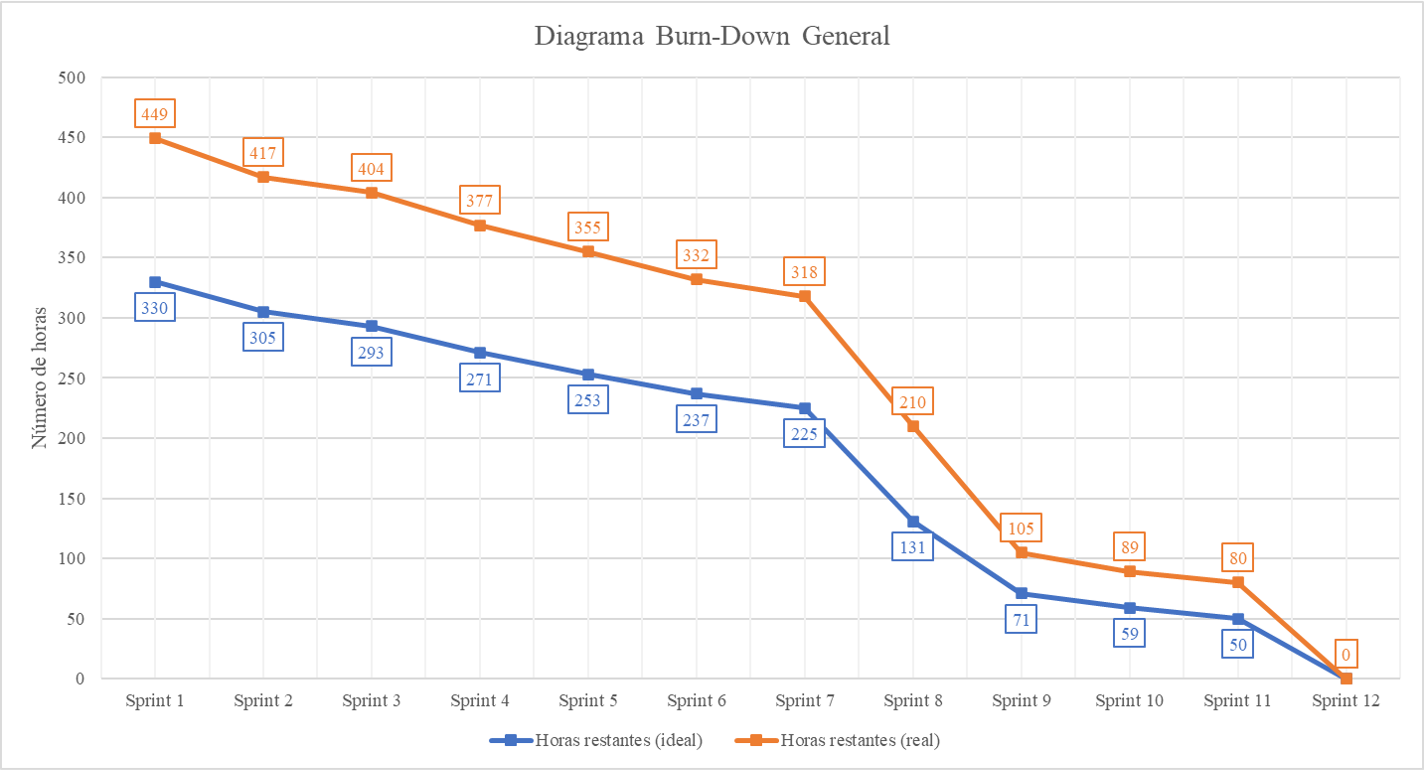
\includegraphics[width=\textwidth]{img/general_burndown_chartpng.png}
	\caption{Diagrama burn-down a nivel de proyecto.}
	\label{fig:general_burndown_chart}
\end{figure}

A la vista de los datos reflejados por el gráfico, se puede observa como a lo largo del proyecto se ha realizado una sobreestimación del esfuerzo requerido para el cumplimiento de las actividades definidas en cada Sprint.

\section{Estudio de viabilidad}

\subsection{Viabilidad económica}

El siguiente apartado tiene como finalidad determinar la viabilidad económica del proyecto, analizando los gastos de inversión necesarios para su desarrollo. En los siguientes secciones se proporciona el desglose de los gastos de personal, gastos hardware y gastos generales requeridos para el desarrollo del proyecto.

\subsubsection{Gastos de personal}

Los gastos de personal representan los gastos que supone contratar al personal requerido para la realización del proyecto. En el caso de nuestro proyecto estos cálculos se realizan considerando que el proyecto ha sido realizado por un único \textbf{programador junior recién egresado}.

El sueldo promedio de un programador junior en España es de \textbf{\numprint{20000} euros brutos anuales} de acuerdo con la información obtenida del portal de la \textbf{Universidad Europea} \cite{ve:salario_ingeniero_informatico}. Realizaremos la estimación de los gastos que supondría mantener a dicho programador a media jornada durante un periodo de 6 meses. En la siguiente tabla se presenta el desglose de los gastos que supondría su contratación.

\tablaSmallSinColores{Desglose de los gastos de personal del proyecto (6 meses)}{l r r}{gastosdepersonal}
{ \multicolumn{1}{l}{\centering\textbf{Concepto}} & \multicolumn{1}{p{2.5cm}}{\raggedleft\textbf{Importe mensual}} & \multicolumn{1}{p{2.5cm}}{\raggedleft\textbf{Importe semestral}} \\}{ 
    \emph{Salario bruto mensual (media jornada)}  & \numprint{833,33} €  & \numprint{5000,00} € \\
    \emph{Contingencias comunes (23,60\%)}        & \numprint{196,67} €  & \numprint{1180,00} € \\
    \emph{Tipo general de desempleo (5,50\%)}     & \numprint{48,83} €   & \numprint{275,00} € \\
    \emph{Fondo de Garantía Salarial (0,20\%)}    & \numprint{1,67} €    & \numprint{10,00} € \\
    \emph{Formación Profesional (0,70\%)}         & \numprint{5,83} €    & \numprint{35,00} € \\ 
    \bottomrule
    \textbf{TOTAL}                                & \numprint{1083,33} € & \numprint{6500,00} € \\
}

\subsubsection{Gastos hardware}

Los gastos hardware se refieren a aquellos dispositivos sobre los que se ha realizado una inversión para cumplir con las necesidades del proyecto. Este tipo de materiales gozan de un periodo de vida útil para el cual se realizan los siguientes cálculos de amortización siguiendo las directrices de los coeficientes de amortización descritos por la Agencia Tributaria \cite{ve:agencia-tributaria-2021}. Se consideran unos costes de amortización por un periodo de \textbf{un año} debido a que el cálculo de este valor se realiza de manera anual.

\tablaSmallSinColores{Desglose gastos hardware del proyecto (Anual)}{l r r}{gastoshardware}
{ \multicolumn{1}{l}{\centering\textbf{Concepto}} & \multicolumn{1}{p{2.5cm}}{\raggedleft\textbf{Importe}} & \multicolumn{1}{p{2.5cm}}{\raggedleft\textbf{Amortización}} \\}{ 
    \emph{Equipo portátil} & \numprint{1000,00} € & \numprint{100,00} € \\
    \emph{Monitor 24''}    & \numprint{150,00} €  & \numprint{15,00} € \\
    \emph{Ratón}           & \numprint{25,00} €   & \numprint{2,50} € \\
    \bottomrule
    \textbf{TOTAL}         & \numprint{1175,00} € & \numprint{117,00} € \\
}

\subsubsection{Gastos generales}

Los gastos generales son aquellos gastos adicionales necesarios para poder llevar a cabo el desarrollo de proyecto. Entre la variedad de supuestos en los que podemos encontrar este tipo de gastos estableceremos una distinción entre aquellos gastos puntuales en materiales específicos requeridos en momentos puntuales, y aquellos gastos de carácter periódico que clasificaremos como gastos de actividad.

En el siguiente desglose se pueden apreciar los gastos material aproximados para cumplir con los requisitos de la entrega de proyecto.

\tablaSmallSinColores{Desglose gastos generales de material del proyecto}{l r}{gastosmaterial}
{ \multicolumn{1}{l}{\centering\textbf{Concepto}} & \multicolumn{1}{p{2.5cm}}{\raggedleft\textbf{Importe}} \\}{
    \emph{Impresión Memoria} & \numprint{30,00} € \\
    \emph{USB 32GB x3}       & \numprint{15,00} € \\
    \bottomrule
    \textbf{TOTAL}           & \numprint{45,00} € \\
}

A continuación, se presenta el desglose de los gastos de actividad surgidos de la necesidad de proporcionar al desarrollador los servicios necesarios para poder cumplir con sus obligaciones durante el desarrollo del proyecto.

\tablaSmallSinColores{Desglose de los gastos generales de actividad del proyecto}{l r r}{gastosactividad}
{ \multicolumn{1}{l}{\centering\textbf{Concepto}} & \multicolumn{1}{p{2.5cm}}{\raggedleft\textbf{Importe mensual}} & \multicolumn{1}{p{2.5cm}}{\raggedleft\textbf{Importe semestral}} \\}{ 
    \emph{Consumo eléctrico}   & \numprint{40,00} €   & \numprint{240,00} € \\
    \emph{Cuota internet}      & \numprint{55,00} €   & \numprint{330,00} € \\
    \emph{Alquiler oficina}    & \numprint{350,00} €  & \numprint{2100,00} € \\
    \emph{Material de oficina} & \numprint{10,00} €   & \numprint{60,00} € \\
    \bottomrule
    \textbf{TOTAL}             & \numprint{455,00} € & \numprint{2730,00} € \\
}

\subsection{Viabilidad legal}

El siguiente apartado tiene como finalidad presentar los aspectos legales del proyecto en referencia a las licencias de uso y distribución de aquellos componentes que conforman el código fuente de la aplicación, así como los relativos a las dependencias y materiales utilizados durante el desarrollo del proyecto.

\subsubsection{Proyecto y Documentación}

El proyecto y su documentación se distribuyen bajo la \textbf{GNU General Public License v3.0} \cite{vl:gplv3} en cumplimiento con las restricciones de uso de aquellos complementos de terceros implicados en el desarrollo y requeridos por la aplicación para su correcto funcionamiento.

La elección de esta licencia de \emph{software libre} responde a la concepción personal de devolver a la comunidad de desarrolladores aquellos conocimientos adquiridos durante su desarrollo. Gracias a los aportes de aquellos desarrolladores que previamente decidieron compartir sus aportes el proyecto ha podido cumplir con los objetivos propuestos.

Las características principales de la licencia \textbf{GNU GPLv3} proporcionan a los futuros interesados en el trabajar con proyecto la capacidad de modificar, distribuir, y utilizar el código tanto de manera comercial, privada o a través de patentes siempre y cuando se incluyan junto con su aplicación el código fuente de este. A su vez, esta licencia exime al creador de ofrecer garantías y responsabilidades sobre el correcto funcionamiento o la aparición de futuros problemas sobre el producto (véase \autoref{fig:gnu-gplv3}).

\begin{figure}[!ht]
	\centering
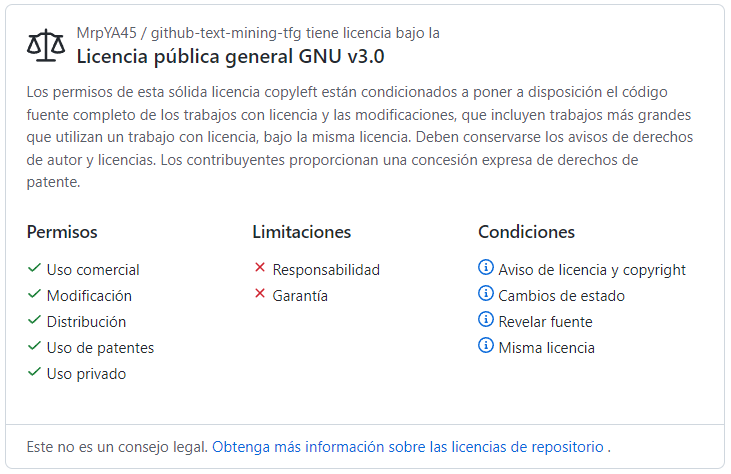
\includegraphics[width=\textwidth]{img/licencia_GNUGPLv3.png}
	\caption{Características de GNU General Public License v3.0 disponibles en el repositorio del proyecto \cite{vl:project-license-2021}.}
	\label{fig:gnu-gplv3}
\end{figure}

\subsubsection{Dependencias}

En esta sección se han recopilado y listado todas aquellas dependencias desarrolladas por terceros de las que se hace uso en el proyecto. Mediante el posterior cuadro se pone en conocimiento los complementos junto con sus correspondientes licencias de derechos de autor de estas para con su uso en el proyecto (véase \autoref{tabla:dependenciaslicencias}).

Todas las licencias incluidas en el proyecto cuentan con el grado necesario de compatibilidad entre ellas y con la propia licencia del proyecto, permitiendo distribuir y modificar el código fuente del proyecto siempre y cuando se mantenga una licencia compatible con todas ellas y con la propia licencia del proyecto.

\tablaSmall{Listado de dependencias con su correspondiente licencia}{p{4.5cm} p{2cm} p{5.2cm}}{dependenciaslicencias}
{ \multicolumn{1}{p{4.5cm}}{\raggedright\textbf{Dependencia}} & \multicolumn{1}{p{2cm}}{\raggedright\textbf{Versión}} & \multicolumn{1}{p{5cm}}{\raggedright\textbf{Licencia}}\\}{ 
    \emph{Python}                           & 3.9.6  & PSF License Agreement \cite{vl:python-software-foundation-2001}\\
    \emph{ReactJS}                          & 17.0.2 & MIT License \cite{vl:mit-license-1988}\\
    \emph{beautifulsoup4}                   & 4.9.3  & MIT License \\
    \emph{blingfire}                        & 0.1.7  & MIT License \\
    \emph{flask}                            & 2.0.1  & BSD-3-Clause Source License \cite{vl:bsd-3-clause-1988}\\
    \emph{flask-cors}                       & 3.0.10 & MIT License \\
    \emph{markdown}                         & 3.3.4  & BSD-3-Clause Source License \\
    \emph{markdown-checklist}               & 0.4.3  & BSD-3-Clause Source License \\
    \emph{mdx-gh-links}                     & 0.2    & BSD-3-Clause Source License \\
    \emph{nltk}                             & 3.6.2  & Apache License 2.0 \cite{vl:apache-2.0-2004}\\
    \emph{numpy}                            & 1.21.2 & BSD-3-Clause Source License \\
    \emph{pygithub}                         & 1.55   & GNU LGPL v3.0 \cite{vl:lgplv3}\\
    \emph{sqlalchemy}                       & 1.4.23 & MIT License \\
    \emph{torch}                            & 1.9.0  & Apache CLA \cite{vl:apache-cla}\\
    \emph{transformers}                     & 4.9.2  & Apache License 2.0 \\
    \emph{react-anchor-link-smooth-scroll}  & 1.0.12 & MIT License \\
    \emph{react google charts}              & 3.0.15 & MIT License \\
    \emph{react-helmet}                     & 6.1.0  & MIT License \\
    \emph{react-toastify}                   & 8.0.1  & MIT License \\
    \emph{react-hook-form}                  & 7.14.0 & MIT License \\
    \emph{wouter}                           & 2.7.4  & ISC License \cite{vl:isc-license-1995}\\
}

